\section{GaitNet}
\label{sec:methodology-gaitnet}

GaitNet is designed to select the optimal footstep action from a
discrete set of candidates. By restricting selection to a predefined
set of continuous actions, the algorithm enforces constraints on the
robot's motion, strictly preventing invalid foot placements and
limiting the range of possible gaits. The inclusion of a no-action
candidate, combined with continuous re-evaluation, distinguishes this
approach: it enables the greedy generation of acyclic gaits in which
multiple feet can be in the swing phase simultaneously.

%%%%%%%%%%%%%%%%%%%%%%%%%%%%%%%%%%%%%%%%%%%%%%%%%%%%%%%%%%%%%%%%%%%%%%%%%%%%%%%%
\subsection{Architecture}
\label{subsec:methodology-gaitnet-architecture}

GaitNet is responsible for ranking footstep candidates based on the
one-hot encoded leg index $\mathbf{f_c}^{\prime}$ and the robot state
$\mathbf{x_g}$:

\[
  \mathbf{x_g} =
  \begin{bmatrix}
    \mathbf p_{b,xy} \\
    \mathbf r_{w,z} \\
    \mathbf v_b \\
    \mathbf \omega_b \\
    \mathbf u \\
    \mathbf g \\
    \mathbf c
  \end{bmatrix}
\]

Descriptions of $\mathbf p_{b,xy}$ and $\mathbf r_{w,z}$ can be found
in \autoref{subsec:methodology-contactnet-architecture}. The
additional terms, compared to the footstep evaluation network, are
$\mathbf g$ and $\mathbf c$. Using $\mathbf{x_g}$ and
$\mathbf{f_c}^{\prime}$, GaitNet outputs a logit associated with each
footstep and the desired swing duration if that step is selected.

\begin{figure}[H]
  \centering
  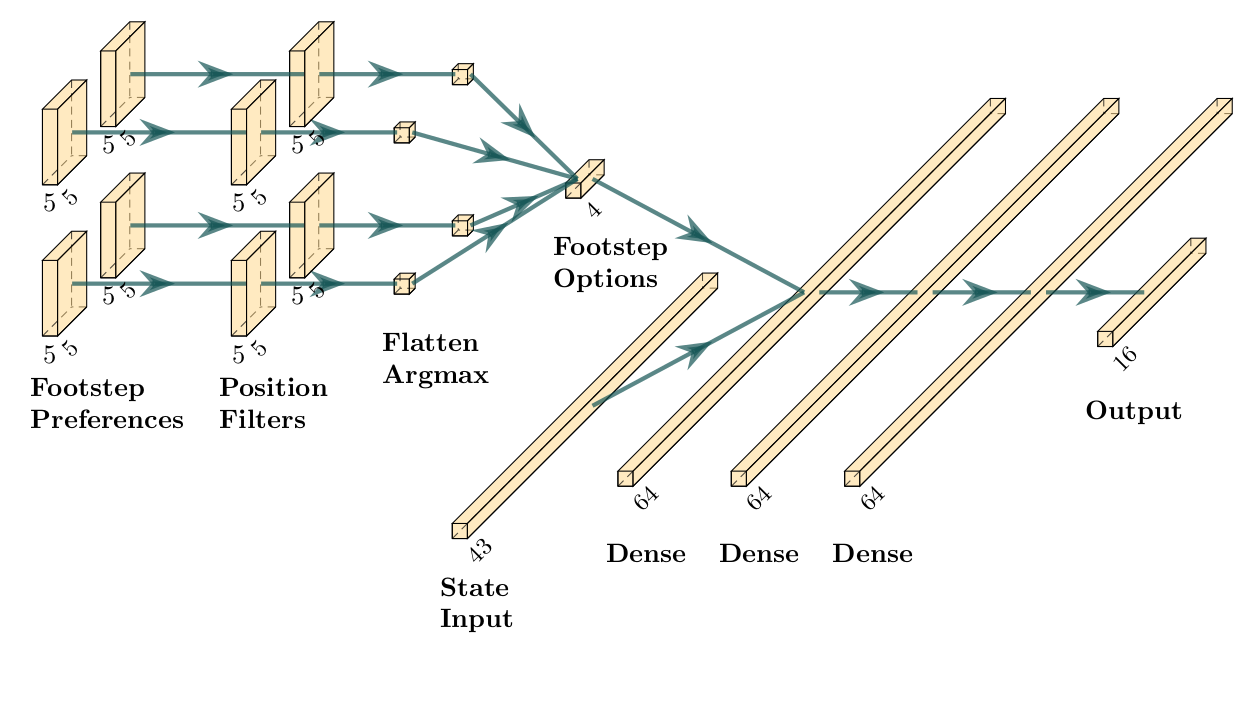
\includegraphics[width=0.625\linewidth]{images/diagrams/gait-network-architecture.png}
  \caption{Gait net architecture. Sections of the diagram include the
    footstep candidate encoder in red,     robot state encoder in blue,
    and shared trunk in green.     The final output is a logit encoding
    the value of this option and the   desired swing duration if this
  action is taken.}
  \label{fig:diagram-gaitnet-architecture}
\end{figure}

The model is designed to jointly evaluate robot state and footstep
candidates with a middle fusion architecture \cite{feng2021deep}. The
architecture (seen in \autoref{fig:diagram-gaitnet-architecture})
consists of two encoders, a shared trunk, and two task-specific output heads:

\begin{itemize}
  \item Robot state encoder: The robot state vector is processed by a
    three-layer feedforward network with intermediate dimensionality
    of 128 and ReLU activations. This produces a fixed-dimensional
    latent representation of the current robot state.
  \item Footstep encoder: Each footstep candidate is encoded by a
    two-layer feedforward network with hidden size 64 and ReLU
    activations. No-action candidates are represented through a fixed embedding.
  \item Shared trunk: The concatenated robot state and footstep
    embeddings are processed by a three-layer feedforward trunk,
    reducing dimensionality while applying Layer Normalization and
    ReLU nonlinearity.
  \item Output heads: Two parallel prediction heads are applied to
    the shared trunk:
    \begin{itemize}
      \item Logit head: A single-layer network outputs the predicted
        reward value as a logit.
      \item Duration head: A single-layer network with sigmoid
        activation outputs a normalized swing duration, which is then
        scaled to the range (0.1, 0.3)\,s.
    \end{itemize}
\end{itemize}

This design allows the network to sequentially evaluate multiple
footstep candidates, assigning each an expected value and a feasible
swing duration, while explicitly supporting a “no-action” option via
a dedicated embedding.

%%%%%%%%%%%%%%%%%%%%%%%%%%%%%%%%%%%%%%%%%%%%%%%%%%%%%%%%%%%%%%%%%%%%%%%%%%%%%%%%
\subsection{Training}
\label{subsec:methodology-gaitnet-training}

Due to the inclusion of the $\mathbf{c}$ term in the input, GaitNet
cannot be effectively trained using supervised learning because of
the high dimensionality of the problem. Instead, it is trained using
PPO \cite{Schulman_proximal_2017}. In this setup, the actor network
is GaitNet (\autoref{fig:diagram-gaitnet-architecture}), while the
critic follows a similar architecture but omits the duration head.
All logits from the critic are passed through a final MLP to produce
a single value estimate. This MLP consists of two hidden layers of
size 64, with ReLU activations applied to all layers except the output.

A custom actor-critic implementation was necessary to handle
GaitNet's dual outputs. The logits define a categorical distribution
over footstep candidates, while the duration output is treated as a
separate normal distribution with a fixed standard deviation of
0.01\,s for each action. To prevent multiple no-action candidates
from skewing the selection, all but one no-action candidate are
removed (set to $-\infty$).

The total log probability of an action is computed as the sum of the
categorical log probability of the selected footstep candidate and
the log probability of the duration under the normal distribution.
During action sampling, a footstep candidate is first sampled from
the categorical distribution, followed by sampling the duration from
its associated normal distribution. The footstep candidate and
duration are then combined to form a complete footstep action.

Following the reward structure, termination conditions, commands, and
hyperparameters outlined in
\autoref{chap:appendix-gaitnet-training-configuration}, GaitNet is
trained for ?? environment steps using a batch size of ??.
